\pagebreak
\section{ПРОГРАММА И МЕТОДИКА ИСПЫТАНИЙ}
\label{sec:testing}

Продемострировать затратность получения информации из файлов возможно несколькими
способами: посчетом числа и времени в необходимых системных вызовах с помощью
\texttt{strace -c}, и подсчетом времени выполнения необязательных функций
утилитой \texttt{perf}. Кроме того, важно при замере производительности
изолировать процесс от воздействия внешних факторов для повышения точности
измерений. К таким факторам относятся непостоянность частоты ЦП ввиду
автоматического подстраивания ее под текущую нагрузку, прерывания, а также
другие процессы на текущем ядре.

В первую очередь, ядро загружается с параметром \texttt{nr\_cpus=1} для нагрузки
по умолчанию только одного ядра процессами.
Отключение изменения частоты процессора можно осуществить записью единицы в
виртуальный файл
\texttt{/sys/devices/system/cpu/intel\_pstate/no\_turbo}. Записью в файлы
\texttt{/proc/irq/*/smp\_affinity} разрешается обработка прерываний только на
нулевом процессоре, после чего при утилитой \texttt{taskset} необходимый
процесс запускается на свободном процессоре.

\begin{figure}
  \centering
  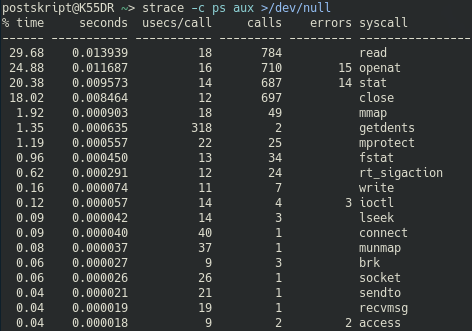
\includegraphics[width=\textwidth]{strace_ps.png}
  \caption{Получение статистики системных вызовов в ps}
  \label{fig:strace_ps}
\end{figure}

На рисунке \ref{fig:strace_ps}
продемонстрирован результат анализа выполнения команды
\texttt{strace -c ps aux}. Полученный результат
показывает, что операции, являющиеся дополнительными действиями из-за работы с
данными через виртуальные файлы и не приносящие никакой полезной информации,
могут занимать до половины времени процесса в пространстве ядра. При этом стоит
учитывать, что полученные таким способом результаты не учитывают временные
затраты на преобразования входных и выходных данных.

Результат работы профилировщика показан на рисунке \ref{fig:perf_report}.
Итоговый суммарный процент времени на дополнительные расходы равен около 20\%.
На высоконагруженных системах такая разница будет значительной, что и было
показано ранее.

\begin{figure}
  \centering
  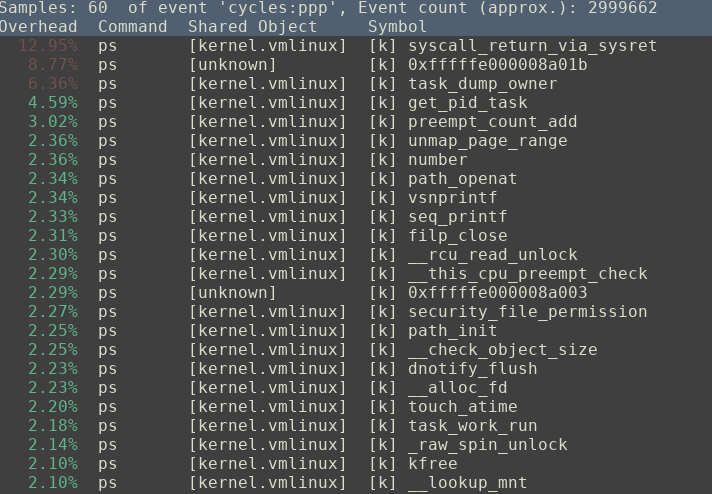
\includegraphics[width=\textwidth]{perf_report.png}
  \caption{Результат анализа производительности}
  \label{fig:perf_report}
\end{figure}
